% !TEX root = ../main.tex
\chapter{绪论} 
\label{chapter:Introduction}

\section{模板概述}
本模板基本结构如下:

\begin{itemize}
\item main.tex: 主文件, 编译对象.
\item figures: 存放论文使用的图片文件夹, 支持多种格式, 直接插入文件名, 不需要输入路径.
\item reference: 存放参考文献文件, 默认为bib文件, 可用bibtex编译得到参考文献.
\item style: 学位论文样式文件, 定义了论文的整体样式.
\item chapter: 章节文件夹, 包含
\begin{itemize}
\item 论文基本信息文件(cover.cfg);
\item 自定义命令文件(defcommands.tex);
\item 摘要(abstract.tex);
\item 正文章节(chapter1.tex, chapter2.tex, conclusions.tex, ...);
\item 在读期间发表的文章(pub.tex);
\item 致谢(thanks.tex).
\end{itemize}
\end{itemize}

\section{编译方式}
本模板支持Windows/Linux/MacOS全平台编译, 编译方式如下:
\begin{enumerate}
\item 安装texlive最新发行版, 如texlive 2023;
\item 使用xelatex编译一次, 然后使用bibtex编译一次, 最后再次使用xelatex编译两次即可.
\end{enumerate}

\section{双语目录与标题}
有些方向要求论文有英文目录或者图表的标题是双语的, 本模板支持双语标题. 调用命令如下:
\begin{verbatim}
\bichapter{中文章节名}{English Chapter Name}
\end{verbatim}
此外, 类似的命令还有: 
\begin{itemize}
\item \verb|\bisection{中文名}{English Name}|
\item \verb|\bisubsection{中文名}{English Name}|
\item \verb|\bisubsubsection{中文名}{English Name}|
\item \verb|\bicaption{中文名}{English Name}|
\end{itemize}

为了生成双语目录, 需要在main.tex中取消\verb|\tableofengcontents|的注释.


\section{插图与引用}
如图 \ref{fig:ASS}.
\begin{figure}[h]
	\centering
	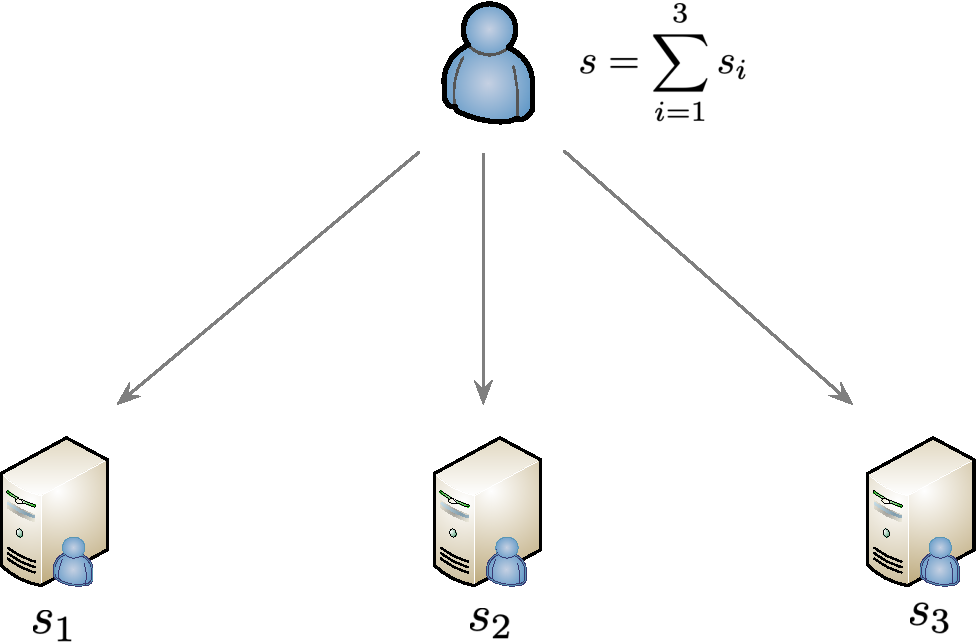
\includegraphics[scale=0.5]{ASS}
	\bicaption{加性秘密共享}{Additive Secret Sharing}
	\label{fig:ASS}
\end{figure}

如果要生成图表的标题目录, 需要在main.tex文件中取消以下两行的注释:
\begin{verbatim}
\listoftables               % 表格目录
\listoffigures              % 插图目录
\end{verbatim}

\section{引用参考文献}
本模板使用bib文件作为参考文献文件, 同时引入了natbib宏包, 此外增添了两个自定义命令:
\begin{itemize}
\item \verb|\citeyearn{citekey}|  ~  引用年份时可在年份后面自动添加``年''
\item \verb|\upcite{citekey}| ~ 上标引用.
\end{itemize}

这是一句测试\cite{Hazay_2010_Efficient}. 引用年份时: \citeyearn{Hazay_2010_Efficient}. 上标引用\upcite{Hazay_2010_Efficient}.

\section{常见问题}
Q1: 如何添加更多章节文件?\\
A1: 按如下步骤操作:
\begin{enumerate}
\item 在chapter文件夹下添加新的tex文件, 例如chapter3.tex
\item 打开main.tex, 在第100行后添加\verb|\include{chapter/chapter3}|
\item 在47-63行的位置, 仿照其他语句加入\verb|chapter/chapter3,|(注意后面有个英文的逗号)
\item 打开chapter3.tex, 第1行输入内容
\begin{verbatim}
% !TEX root = ../main.tex
\end{verbatim}
从第2行开始输入正文.
\item 编译查看结果.
\end{enumerate}

Q2: 如何修改论文作者信息?\\
A2: 直接修改cover.cfg文件中的信息.\\

Q3: 如何加入自定义命令和宏包?\\
A3: 请在defcommands.tex中添加自定义命令和宏包.\\

Q4: 可否修改为硕士学位论文?\\
A4: 在main.tex文件中将语句\verb|\phdtrue|注释掉, 同时取消\verb|\phdfalse|的注释. 默认为博士学位论文. (目前似乎还有些BUG, 正文页眉不会随之改变, 待修正)\\

Q5: 如何生成盲审论文?\\
A5: 首先确保main.tex文件中的第48行这个\verb|\includeonly|命令中正确包含了需要盲审的章节, 然后按如下步骤操作:
\begin{enumerate}
\item 在main.tex文件中注释掉\verb|\blindfalse|, 打开\verb|\blindtrue|
\item 取消\verb|\linenumbers|的注释, 正文部分每隔5行自动生成一个行号
\item 使用xelatex编译3次生成盲审结果
\end{enumerate}

Q6: 能否生成不同版本号用来区分不同的版本?\\
A6: 打开cover.cfg, 在\verb|\version{}|中填写需要的版本号, 如此, 将在首页生成一个版本号信息. 本模板提供了自定义了一个日期时间作为版本号, 调用方式为输入\verb|\version{\today}|, 结果如同(版本: \today). 当然, 版本号可以修改为任意其他文字, 例如定稿时, 修改为``终稿''.
